\documentclass[12pt]{article}

\usepackage[default]{lato}
\usepackage[T1]{fontenc}
\usepackage{graphicx}
\usepackage{blindtext}

\usepackage{tikz}
\usetikzlibrary{positioning, matrix, arrows.meta,calc}

\usepackage[font=small,labelfont=bf, justification=justified, format=plain]{caption}
\tolerance=1
\emergencystretch=\maxdimen
\hyphenpenalty=10000
\hbadness=10000

\renewcommand{\contentsname}{Spis treści}
\renewcommand{\figurename}{Ilustracja nr.}

\usepackage[margin=2cm]{geometry}


\title{}
\author{}
\date{}

\begin{document}
	\begin{titlepage}
		\centering
		\vspace{1cm}
		{\huge\bfseries Systemy cyfrowe i komputerowe\par}
		\vspace{0.5cm}
		{\huge\bfseries Dokumentacja projektu ``exe\_unit\_w1''\par}
		\vspace{2cm}
		{\Large\itshape Karol Ambroziński\par}
		\vspace{0cm}
		{\Large\itshape Nr. albumu: 318488\par}
		\vfill
	\end{titlepage}

	\tableofcontents
	
	\newpage
	
	\section{Wejścia, wyjścia, parametry i zakresy ich wartości}
	
	\subsection{Parametry}
\begin{itemize}
	\item \emph{\textbf{m}} - określa wielkość w bitach główne wejścia i wyjścia danych,
	\item \emph{\textbf{n}} - określa ilość operacji.
\end{itemize}

\subsection{Wejścia}

\begin{itemize}
	\item \emph{\textbf{i\_oper}} - n-bitowe wejście określające wykonywaną operację,
	\item \emph{\textbf{i\_argA}} - m-bitowe wejście; kodowanie ZNAK-MODUŁ,
	\item \emph{\textbf{i\_argB}} - m-bitowe wejście; kodowanie ZNAK-MODUŁ,
	\item \emph{\textbf{i\_clk}} - 1 bitowe wejście zegarowe,
	\item \emph{\textbf{i\_rsn}} - 1 bitowe wejście resetu synchronicznego.
\end{itemize}

\subsection{Wyjścia}
\begin{itemize}
	\item \emph{\textbf{o\_status}} - m-bitowe wyjście,
	\item \emph{\textbf{o\_result}} - 4 bitowe wyjście; kodowanie ZNAK-MODUŁ lub U2.
\end{itemize}


	
	\section{Realizowane funkcje i ich argumenty}

	Układ realizuje 4 operacje (4 podmoduły):

\subsection{Podmoduł \emph{mod1}:}
Odejmowanie argumentów (A - B); jeśli operacja nie może zostać wykonana, jednostka zgłasza błąd, a wyjście jest niezdefiniowane.

\subsubsection*{Wejścia}
\begin{itemize}
	\item i\_argA - m-bitowe wejście,
	\item i\_argB - m-bitowe wejście,
\end{itemize}
\subsubsection*{Wyjścia}
\begin{itemize}
	\item o\_result - m-bitowe wyjście,
	\item o\_status - 4 bitowe wyjście.
\end{itemize}

\subsection{Podmoduł \emph{mod2}:}
Porównanie argumentów (A < B); jeśli warunek jest spełniony to wynikiem jest liczba 1, w przeciwnym wypadku wynikiem jest 0,

\subsubsection*{Wejścia}
\begin{itemize}
	\item i\_argA - m-bitowe wejście,
	\item i\_argB - m-bitowe wejście,
\end{itemize}
\subsubsection*{Wyjścia}
\begin{itemize}
	\item o\_result - m-bitowe wyjście,
	\item o\_status - 4 bitowe wyjście.
\end{itemize}

\subsection{Podmoduł \emph{mod3}:}
Ustawienie bitu w argumencie A na wartość 0; numer bitu jest określony w argumencie B; zgłoszenie błędu jeśli wartość B jest ujemna lub przekrasza liczbę bitów argumentu A,

\subsubsection*{Wejścia}
\begin{itemize}
	\item i\_argA - m-bitowe wejście,
	\item i\_argB - m-bitowe wejście,
\end{itemize}
\subsubsection*{Wyjścia}
\begin{itemize}
	\item o\_result - m-bitowe wyjście,
	\item o\_status - 4 bitowe wyjście.
\end{itemize}

\subsection{Podmoduł \emph{mod4}:}
Konwersja argumentu A z kodu ZNAK-MODUŁ na U2; jeśli konwersja nie może zostać wykonana - zgłaszany jest błąd a wynik jest nieokreślony.

\subsubsection*{Wejścia}
\begin{itemize}
	\item i\_argA - m-bitowe wejście,
\end{itemize}
\subsubsection*{Wyjścia}
\begin{itemize}
	\item o\_result - m-bitowe wyjście,
	\item o\_status - 4 bitowe wyjście.
\end{itemize}
	
	\section{Schemat blokowy struktury jednostki}
	
		\begin{figure}[htb]
	\centering
	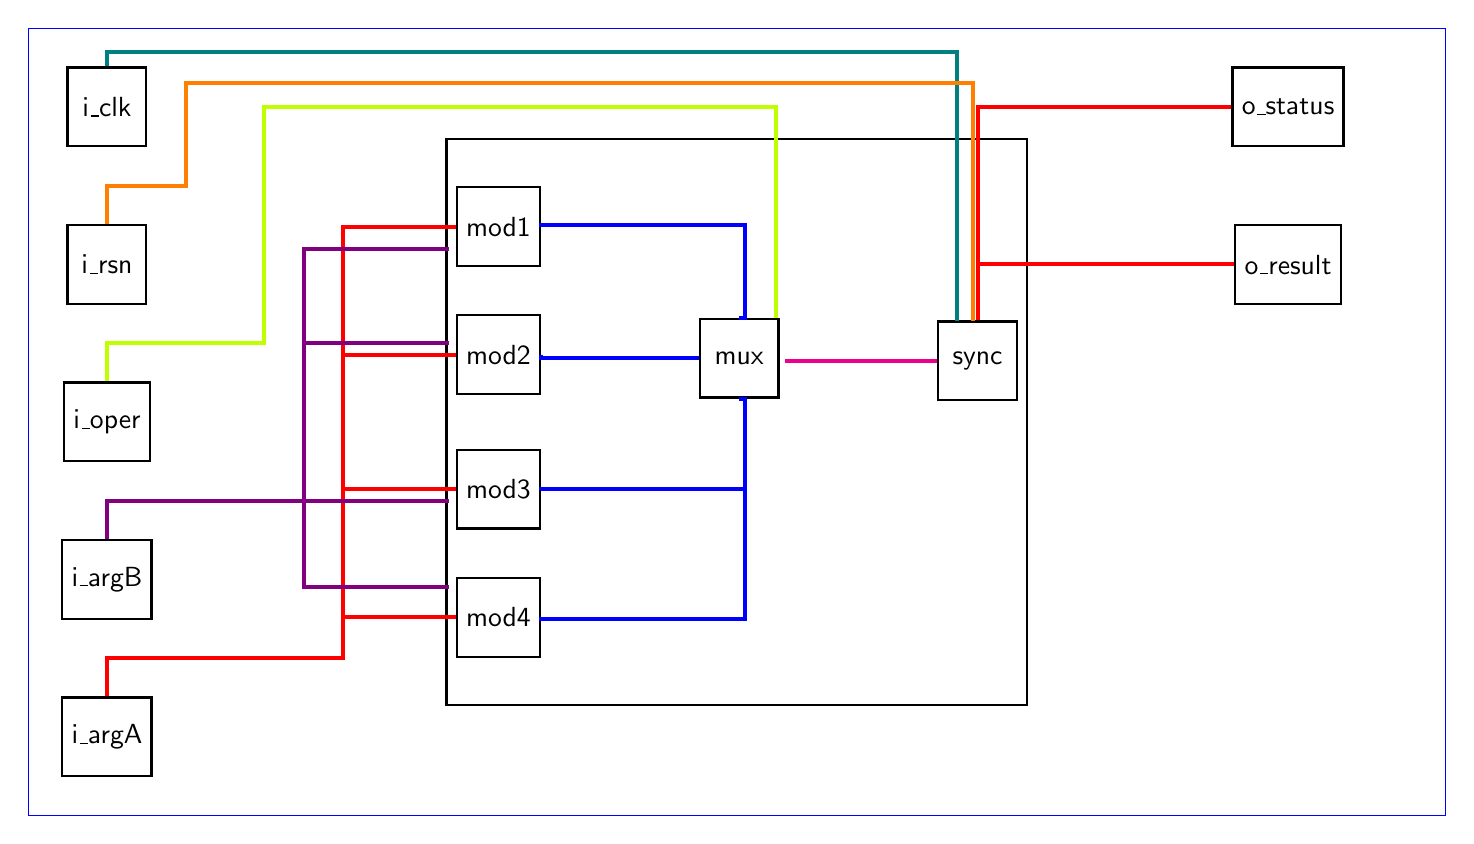
\begin{tikzpicture}[
		myline/.style={draw=black!40!black, thick},
		box/.style={myline, minimum height=1cm, minimum width=1cm, font=\sffamily, inner sep=.3333em}, >=Stealth]
		
		\draw [blue] (-11,-1) rectangle (7,9);
		
		\matrix (ALU) [matrix of nodes, inner ysep=6mm, nodes=box, myline, column sep=20mm, row sep = 6mm] at (-2,4)
		{|(mod1)|mod1 \\ |(mod2)|mod2 & |(mux)|mux & |(sync)|sync \\ |(mod3)|mod3 \\ |(mod4)|mod4 \\};
		
		
		
		\node[box] at (-10,0)  (argA) {i\_argA};
		\node[box] at (-10, 2) (argB) {i\_argB};
		\node[box] at (-10,4)  (oper) {i\_oper};
		\node[box] at (-10,6)  (rsn) {i\_rsn};
		\node[box] at (-10,8)  (clk) {i\_clk};
		
		\node[box] at (5,6)  (result) {o\_result};
		\node[box] at (5,8)  (status) {o\_status};
		
		\draw[-, red, line width=0.5mm]  (argA)|-(-10, 1)|-(-7, 1)|-(-7, 6)|-(mod1);
		\draw[-, red, line width=0.5mm]  (argA)|-(-10, 1)|-(-7, 1)|-(-7, 4)|-(mod2);;
		\draw[-, red, line width=0.5mm]  (argA)|-(-10, 1)|-(-7, 1)|-(-7, 2)|-(mod3);
		\draw[-, red, line width=0.5mm]  (argA)|-(-10, 1)|-(-7, 1)|-(-7, 1)|-(mod4);
		\draw[-, red, line width=0.5mm]  (sync)|-(result);	
		\draw[-, red, line width=0.5mm]  (sync)|-(status);
		
		\draw[-, red, line width=0.5mm]  (argA)|-(-10, 1)|-(-7, 1)|-(-7, 6)|-(mod1);
		\draw[-, red, line width=0.5mm]  (argA)|-(-10, 1)|-(-7, 1)|-(-7, 4)|-(mod2);
		\draw[-, red, line width=0.5mm]  (argA)|-(-10, 1)|-(-7, 1)|-(-7, 2)|-(mod3);
		\draw[-, red, line width=0.5mm]  (argA)|-(-10, 1)|-(-7, 1)|-(-7, 1)|-(mod4);
		
		%\draw[-, blue, line width=0.5mm]  (argB)|-(-10, 3)|-(-7.5, 3)|-(-7.5, 3)|-(-7.5, 1.8)|-(-5.64, 1.8);
		%\draw[-, violet, line width=0.5mm]  (argB)|-(-10, 3)|-(-7.5, 3)
		\draw[-, violet, line width=0.5mm]  (argB)|-(-10, 3)|-(-7.5, 3)|-(-7.5, 1.9)|-(-5.65, 1.9);
		\draw[-, violet, line width=0.5mm]  (argB)|-(-10, 3)|-(-7.5, 3)|-(-5.65, 3);
		\draw[-, violet, line width=0.5mm]  (argB)|-(-10, 3)|-(-7.5, 3)|-(-7.5, 5)|-(-5.65, 5);
		\draw[-, violet, line width=0.5mm]  (argB)|-(-10, 3)|-(-7.5, 3)|-(-7.5, 6.2)|-(-5.65, 6.2);;
		
		\draw[-, lime, line width=0.5mm]  (oper)|-(-8, 5)|-(-8, 8)|-(-1.5, 8)|-(-1.5, 5.32);
		
		\draw[-, teal, line width=0.5mm]  (clk)|-(-8, 8.7)|-(0.8, 8.7)|-(0.8, 5.28);
		
		\draw[-, orange, line width=0.5mm]  (rsn)|-(-9, 7)|-(-9, 8.3)|-(1, 8.3)|-(1, 5.28);
		
		\draw[-, magenta, line width=0.5mm]  (-1.37,4.75)|-(sync.west);
		\draw[-, blue, line width=0.5mm]  (mod2.east)|-(mux);
		\draw[-, blue, line width=0.5mm]  (mod3.east)|-(-1.9, 3.15)|-(mux.south);
		\draw[-, blue, line width=0.5mm]  (mod4.east)|-(-1.9, 1.5)|-(mux.south);
		\draw[-, blue, line width=0.5mm]  (mod1.east)|-(-1.9, 6.5)|-(mux.north);
	\end{tikzpicture}
	\caption{Schemat blokowy \textbf{\emph{exe\_unit\_w1}}}
\end{figure}
	
	\section{Sygnały zaimplementowanych flag i ich wartości}
	
	Zaimplementowane flagi o\_status:

\begin{itemize}
	\item ERROR - operacja nie została wykonana - o\_result jest nieokreślone; pierwszy bit o\_status od prawej jest równy 1,
	\item NEG - wynik jest liczbą ujemną; drugi bit o\_status od prawej jest równy 1,
	\item EVEN - w wyniku jest parzysta liczba jedynek; trzeci bit o\_status od prawej jest równy 1,
	\item ONES - wszystkie bity o\_result ustawione; ostatni bit o\_status od prawej jest równy 1,
\end{itemize}

\noindent
Jeśli wynik jest nieokreslony (flaga ERROR) to pozostałe bity nie są ustawiane; warunki pozostałych flag nie są sprawdzane.

	\newpage

	\section{Przykład użycia modułu}
	\blindtext
	\section{Lista plików}
	\blindtext
	\section{Raport z syntezy logicznej}
	\blindtext
	\section{Raport z symulacji układów}
	\blindtext
	
\end{document}